\documentclass[a4paper,12pt]{article} % Tipo de documento y tamaño de letra.
\usepackage[utf8]{inputenc} % Para que reconozca caracteres especiales como tildes.
\usepackage[spanish]{babel} % Para definir el idioma y el formato de fechas en español.
\usepackage{amsmath, amssymb} % Paquetes para símbolos y ecuaciones avanzadas (Para hacer una ecuación con un recuadro).
\usepackage{ragged2e}
\usepackage{multicol} % Para crear columnas.
\usepackage{slashed} % Para generar números o variables canceladas (Una línea diagonal sobre el número o variable)
\usepackage{graphicx} % Paquete para poner graficas.
\usepackage{float} % Para poder dejar la imagen en un punto fijo del documento.


\title{Actividad Grupal.} 
\author{Liz Ángel Núñez Torres.
Marcos Peñate Sanchéz.} 
\date{\today} 

\begin{document}

\maketitle 

\section*{Problema 1} % Comienza la primera sección.

\begin{justify}
    Un hombre está de pie a un metro del borde de un disco giratorio inmenso, de \(50 \; m.\) de radio. El disco gira a \(1 \; rad/s.\) Calcula y explica:
\end{justify}

\begin{enumerate}
    \item Coeficiente de rozamiento mínimo que tiene que haber entre el suelo y los zapatos del hombre para que se mantenga quieto y no salga despedido.
    \item ¿Qué le sucedería al hombre si avanza un metro hacia el centro del disco?
    \item ¿Qué le sucedería al hombre si se aleja medio metro del centro del disco?
\end{enumerate}

\vspace{\baselineskip}

\subsection*{Solución.}

\begin{justify}
    \textbf{Datos:}
\end{justify}

\begin{multicols}{2}
    \(r = 50 \; m.\)
    
\columnbreak
    \(\omega = 1 \; rad/s.\)
    
\end{multicols}

\begin{justify}
    \textbf{(1)} Como el hombre esta a un metro del borde, tendremos que el radio donde esta ubicado es \(\rightarrow r = 49.\)
\end{justify}

\begin{justify}
    El hombre experimenta dos fuerzas, la fuerza centrípeta \(F_c\) que actua al centro del disco, y la fuerza de rozamiento \(F_r\) que contrarrestra su trayectoria tangencial al disco (Primera ley de Newton).
\end{justify}

\newpage


\begin{justify}
    Para que se el sujeto se mantenga en su sitio la fuerza de rozamiento deberá ser mayor o igual a la fuerza centrípeta.
\end{justify}


\begin{center}
    \(F_r \geq  F_c.\)
\end{center}

\vspace{\baselineskip}


\begin{justify}
    Dado que queremos obtener el valor mínimo de rozamiento trabajaremos de la forma:
\end{justify}

\begin{center}
    \(F_r = F_c.\)
\end{center}

\vspace{\baselineskip}

\begin{justify}
    Donde necesitaremos saber la equivalencia de las fuerzas y otros datos:
\end{justify}

\begin{multicols}{4}
    \(F_r = \mu \cdot N. \)

    \columnbreak

    \(F_c = m \cdot a_c.\)

    \columnbreak

    \(N = m \cdot g.\)

    \columnbreak

    \(a_c = \omega^2 \cdot r. \)
\end{multicols}

\vspace{\baselineskip}

\begin{justify}
    Procedemos a buscar entonces nuestro valor mínimo de fricción.
\end{justify}

\(F_r = F_c \hspace{0.5 cm}  \Longrightarrow \hspace{0.5 cm}  \mu \cdot N = m \cdot a_c  \hspace{0.5 cm}  \Longrightarrow \hspace{0.5 cm} \mu \cdot m \cdot g = m \cdot \omega^2 \cdot r \)

\vspace{\baselineskip}

\begin{center}
    \( \mu = \frac{\slashed{m} \cdot \omega^2 \cdot r }{\slashed{m} \cdot g}\hspace{0.5 cm}  \Longrightarrow \hspace{0.5 cm} \mu = \frac{\omega^2 \cdot r}{g}.\)
\end{center}

\vspace{\baselineskip}

\begin{justify}
    Reemplazamos en la ecuación obtenida los datos dados en el problema: 
\end{justify}

\begin{center}
    \(\mu = \frac{1^2 \cdot 49}{9.81} = 4.99.\)
\end{center}

\vspace{\baselineskip}

\begin{justify}
    El valor mínimo de fricción para que el sujeto permanezca en el disco es:
\end{justify}

\begin{center}
    \[
    \boxed{\mu = 4.99.}
    \]
\end{center}

\newpage

\begin{justify}
    \textbf{(2)} Vamos a ver que sucede si el hombre avanza un metro hacia el centro del disco desde el punto en que calculamos anteriormente la fricción \(\mu.\)
\end{justify}

\begin{justify}
    Usaremos la ecuación obtenida anteriormente y reemplazaremos con los nuevos datos.
\end{justify}

\begin{center}
    \[
    \boxed{\mu = \frac{1^2 \cdot 48}{9.81} = 4.89.}
    \]
\end{center}

\begin{justify}
    Cuando el sujeto se desplaza un metro hacia dentro, la fuerza de fricción que se debe efectuar para mantenerlo en el disco es menor.
\end{justify}

\vspace{\baselineskip}

\begin{justify}
    \textbf{(3)} A continuación, analizaremos que le sucedería al sujeto si estando en el centro del disco se aleja medio metro del mismo.
\end{justify}

\begin{justify}
    Para esto, usaremos la ecuación obtenida en el punto \textbf{(1)} además de ajustar el valor del radio \(r = 0.5.\)
\end{justify}

\begin{center}
    \[
    \boxed{\mu = \frac{1^2 \cdot 0.5}{9.81} = 0.0509.}
    \]
\end{center}

\begin{justify}
    Igual que en el punto \textbf{(2)} la fuerza de fricción necesaria para mantener el sujeto en el disco es menor, por esto, podemos argüir que la fuerza de fricción es directamente proporcional al radio de la circunferencia, dado que al diminuir el radio también disminuye la fuerza de fricción.  
\end{justify}

\newpage 

\section*{Problema 2} % Comienza la segunda sección.

\begin{figure}[h!]
    \centering
    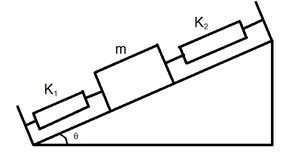
\includegraphics[width=\textwidth]{Imagen actividad G.jpg}
    \caption{El bloque de la figura se encuentra en equilibrio, sujeto por ambos resortes. }
\end{figure}

\begin{justify}
    \textbf{Los datos de cada elemento son los siguientes:}
\end{justify}

\begin{itemize}
    \item Constantes recuperadoras de los muelles: \(K_1 = 70 \; N/m \Longrightarrow K_2 = 50 \; N/m.\)
    \item Masa del cuerpo \(\hspace{0.5 cm} \Longrightarrow \hspace{0.5 cm} m = 10 \; kg.\)
    \item Longitudes originales de los dos muelles \(\hspace{0.5 cm} \Longrightarrow \hspace{0.5 cm} L = 1 \; m.\)
    \item Ángulo de inclinación del plano \(\hspace{0.5 cm} \Longrightarrow \hspace{0.5 cm} \theta = 30. \)
\end{itemize}

\vspace{\baselineskip}

\begin{enumerate}
    \item Con estos datos calcula la posición de equilibrio del bloque, esto es, cuánto se comprime el de abajo, o lo que es lo mismo, que se estire el de arriba.
\end{enumerate}

\subsection*{Solución.}

\begin{justify}
    \textbf{Hacemos el diagrama de cuerpo libre:}
\end{justify}

\begin{figure}[H]
    \centering
    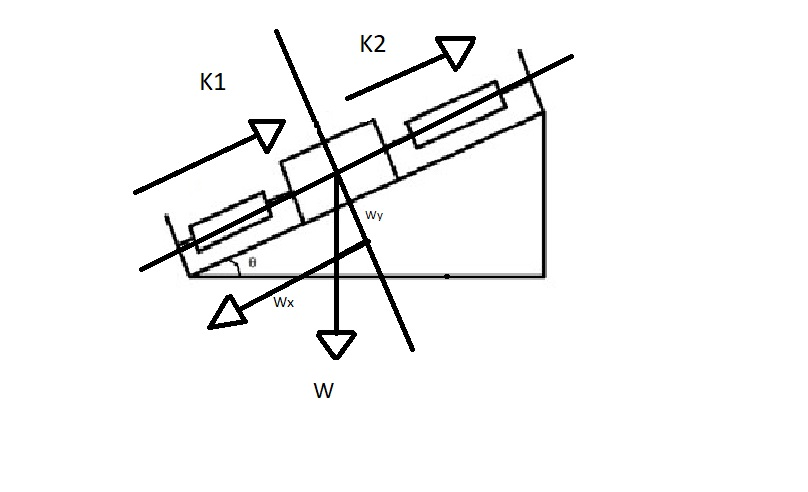
\includegraphics[width=\textwidth]{Diagrama de cuerpo libre.jpg}
    \caption{DLC. }
\end{figure}

\begin{justify}
    El resorte \(K_1\) es comprimido mientras el resorte \(K_2\) ha sido  estirado, por esto en el diagrama de fuerzas ambos vectores tienen la misma dirección y sentido. 
\end{justify}

\begin{itemize}
    \item \(K_1\) emplea una fuerza para recuperar su forma de la compresión que ejerce el bloque. 
    \item \(K_2\) emplea una fuerza para comprimirse del estiramiento que ejerce el bloque. 
    \item El vector \(W_x\) va en dirección y sentido contrario al de los resortes, tal como vemos en el diagrama de cuerpo libre, donde descomponemos \(W\) en sus vectores suma (Hemos exagerado el módulo de \(W_x\) para mostrar el sentido del vector).
\end{itemize}

\newpage

\begin{justify}
    Recordemos que al hablar de resortes debemos aplicar la \textbf{Ley de Hooke} que establece que la fuerza aplicada a un cuerpo es directamente proporcional a su deformación, y se expresa matemáticamente como:
\end{justify}

\begin{center}
    \(F = k \cdot x.\)
\end{center}

\begin{justify}
    Dado que el bloque está en equilibrio, quiere decir que se está aplicando la primera Ley de Newton.
\end{justify}

\begin{center}
    \(\Sigma F = 0.\)
\end{center}

\begin{justify}
    En nuestro caso:
\end{justify}

\begin{center}
    \(K_1 + K_2 - W_x = 0.\)
\end{center}
\begin{justify}
    Vamos a sustituir nuestra variables y proceder con la ecuación.
\end{justify}

\(k_1 \cdot x + k_2 \cdot x - m \cdot g \cdot sin\;\theta  \Longrightarrow x \left(k_1 + k_2\right) = m \cdot g \cdot sin \; \theta .\)

\begin{center}
    \[{x = \frac{ m \cdot g \cdot sin \; \theta }{k_1 + k_2}}.\]
\end{center}

\begin{justify}
    Reemplazamos por los datos:
\end{justify}

\begin{center}
    \[
    \boxed{x =\frac{10 \cdot 9.81 \cdot 0.5}{70+50} = 0.408 \; m. }
    \]
\end{center}

\begin{itemize}
    \item Por lo tanto, podemos afirmar que el resorte \(K_1\) se comprime \( 0.408 \; m.\) y el resorte \(K_2\) se expande \( 0.408 m.\)
\end{itemize}

\newpage

\newpage

\section*{Problema 3}
\begin{figure}[h!]
    \centering
    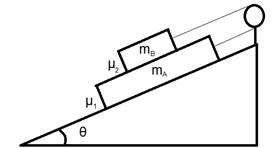
\includegraphics[width=\textwidth]{Imagen2.jpg}
    \caption{Dos bloques de madera se encuentran sobre un plano inclinado, unidos por una polea y una cuerda de masas y efectos despreciables.}
\end{figure}

\begin{justify}
    \textbf{Los datos de cada elemento son:}
\end{justify}

\begin{itemize}
    \item Masas de los bloques \(\hspace{0.5 cm}  \Longrightarrow  \hspace{0.5 cm} m_A = 20 \; kg. \hspace{0.5 cm} m_B = 10.\)
    \item Coeficiente  de rozamiento entre el plano y la masa \(A  \Longrightarrow \hspace{0.5 cm} \mu_1 = 0.2.\)
    \item Coeficiente de rozamiento entre las masas \(A\) y \(B   \Longrightarrow  \hspace{0.5 cm} \mu_2 = 0.3.\)
    \item Ángulo del plano inclinado \(\hspace{0.5 cm} \Longrightarrow \hspace{0.5 cm} 50.\)
\end{itemize}

\begin{justify}
    \textbf{Calcular:}
\end{justify}

\begin{enumerate}
    \item Aceleración y su sentido.
    \item Si el centro del bloque \(B\) está a \(50 \; cm.\) de cada uno de los bloques (dicho de otro modo, que el bloque \(A\) mide \(1 \; m.\)), calcular el tiempo que tarda el centro del bloque \(B\) en llegar al borde.
    \item Valor del ángulo que impediría el movimiento de los bloques. 
\end{enumerate}


\subsection*{Apartado 1}

\begin{justify}
    El sistema tiene dos bloques, \( A \) sobre el plano y \( B \) sobre el bloque \( A \). Las fuerzas en juego son:    
\end{justify}

\begin{justify}
    Para el bloque \( A \):    
\end{justify}

\begin{itemize}
    \item Peso \( F_{g_A} = M_A \cdot g \)
    \begin{itemize}
        \item Componente paralela al plano: \( F_{A,\parallel} = M_A \cdot g \cdot \sin(\theta) \)
        \item Componente perpendicular al plano: \( F_{A,\perp} = M_A \cdot g \cdot \cos(\theta) \)
    \end{itemize}
    \item Normal que incluye el peso de \( M_B \): \( N = (M_A + M_B) \cdot g \cdot \cos(\theta) \)
    \item Fricción: \( F_f = \mu \cdot N \)
\end{itemize}

Para el bloque \( B \):
\begin{itemize}
    \item Ejerce fricción adicional sobre el bloque \( A \): \( F = \mu_2 \cdot M_B \cdot g \)
\end{itemize}

La fuerza neta que genera aceleración en el sistema es la suma de las fuerzas paralelas al plano menos las de fricción. Por lo tanto, la aceleración es:

\[
F_{\text{tot}} = M_A \cdot g \cdot \sin(\theta) - \mu_1 \cdot (M_A + M_B) \cdot g \cdot \cos(\theta) - \mu_2 \cdot M_B \cdot g
\]

Como sabemos \( F = m \cdot a \), ergo:

\[
a = \frac{F_{\text{tot}}}{M_A + M_B}
\]

Sustituimos los valores dados:
\[
F_{A,\parallel} = 20 \cdot 9.8 \cdot 0.766 = 150.1 \, \text{N}
\]
\[
F_f = 0.2 \cdot (20 + 10) \cdot 9.8 \cdot 0.643 = 37.8 \, \text{N}
\]
\[
F_{f,2} = 0.3 \cdot 10 \cdot 9.8 = 29.4 \, \text{N}
\]

Por tanto, la aceleración es:

\[
a = \frac{82.9}{20 + 10} \approx 2.76 \, \text{m/s}^2
\]

De lo que deducimos que es hacia abajo, ya que la fuerza neta es positiva en esa dirección.

\subsection*{Apartado 2}
La distancia recorrida por el bloque \( A \) se puede calcular con la ecuación de movimiento rectilíneo uniformemente acelerado (MRUA) en la dirección paralela al plano inclinado:

\[
d = d_0 + v_0 t + \frac{1}{2} a t^2
\]

Por lo que, asumiendo que empieza en reposo, el tiempo que tarda \( B \), sabiendo su aceleración y la distancia que recorrerá \( A \), es:

\[
t = \sqrt{\frac{2 \cdot 0.5}{2.76}} \approx 0.6 \, \text{s}
\]

\subsection*{Apartado 3}
El ángulo que haría que los bloques no se muevan es aquel que les dejará en equilibrio, es decir, que la fuerza neta sea \( 0 \). Por lo tanto, la fuerza de fricción debe ser igual a la componente paralela al plano inclinado:

\[
F_{A,\parallel} = F_{f,1} + F_{f,2}
\]

\[
\tan(\theta) = \frac{\mu_1 \cdot (M_A + M_B) + \mu_2 \cdot M_B}{M_A}
\]

\[
\tan(\theta) = \frac{0.2 \cdot (20 + 10) + 0.3 \cdot 10}{20} = 0.45
\]

Resolvemos y obtenemos que el ángulo que haría que el objeto se mantuviese inmóvil sería:

\[
\theta = \arctan(0.45) \approx 24.22^\circ
\]


\section*{Problema 4}

\begin{justify}
    \textbf{Resuelve el siguiente problema utilizando el principio de conservación de la energía.}
\end{justify}
\begin{figure}[h!]
    \centering
    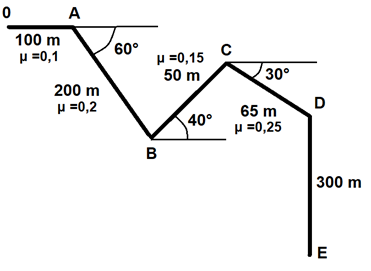
\includegraphics[width=\textwidth]{problema 4.png}
    \caption{Un bloque de 100 kg. de masa parte del punto 0 de la figura a una velocidad de 100 m/s y recorre el circuito de la figura.}
\end{figure}

\begin{enumerate}
    \item Las velocidades del cuerpo en los puntos \(A, B, C, D\) y \(E\).
    \item Las velocidades del cuerpo en los puntos \(B, C, D\) y \(E\) si consideramos que el cuerpo perdió, al llegar al punto \(B\), el \(10\%\) de su energía mecánica.
\end{enumerate}

\subsection*{Apartado 1}
El diagrama da la medida de cada tramo, no su altura, y un ángulo respecto a la horizontal, por lo que usaremos la fórmula:
\[
\Delta h = L \cdot \sin(\theta).
\]
Se sabe que:
\begin{itemize}
    \item $h_e = 0\,\mathrm{m}$,
    \item $h_d = 300\,\mathrm{m}$,
    \item $h_c = h_d + 32.5 \approx 332.5\,\mathrm{m}$ ya que $\theta_{c \to d} = 30^\circ$,
    \item $h_b \approx 300\,\mathrm{m}$ ya que está por debajo de $C$ subiendo $50\,\mathrm{m}$ con ángulo de $40^\circ$,
    \item $h_a \approx 473\,\mathrm{m}$ subiendo $200\,\mathrm{m}$ con ángulo $60^\circ$ desde $B$,
    \item $h_0 = h_a$, por lo que $h_0 = 473\,\mathrm{m}$.
\end{itemize}

Con estos cálculos sabemos que el bloque parte de $h_0 = 473\,\mathrm{m}$ con una velocidad de $100\,\mathrm{m/s}$.

La energía mecánica se conserva en el sistema, por lo que la energía cinética inicial más la energía potencial inicial es igual a la energía cinética final más la energía potencial final.

La energía inicial es:
\[
E_i = C_i + P_i,
\]
\[
E_i = \frac{1}{2} m v_0^2 + m g h_0,
\]
\[
E_i \approx \frac{1}{2} \cdot 100 \cdot 100^2 + 100 \cdot 9.8 \cdot 473,
\]
\[
E_i = 500000\,\mathrm{J} + 463540\,\mathrm{J} = 963540\,\mathrm{J}.
\]

Para el tramo $0 \to A$:
\[
N = m \cdot g \cdot \cos(0) = 100 \cdot 9.8 \cdot 1 = 980\,\mathrm{N},
\]
\[
F_f = \mu \cdot N = 0.1 \cdot 980 = 98\,\mathrm{N},
\]
\[
W_f = 98 \cdot 100 = 9800\,\mathrm{J},
\]
\[
E_a = E_i - W_f = 963540 - 9800 = 953740\,\mathrm{J},
\]
\[
E_p = 100 \cdot 9.8 \cdot 473 = 463540\,\mathrm{J},
\]
\[
E_c = E_a - E_p,
\]
\[
E_c = 953740 - 463540 = 490200\,\mathrm{J},
\]
\[
490200 = \frac{1}{2} m v^2,
\]
\[
v = 99\,\mathrm{m/s}.
\]

Para el tramo $A \to B$:
\[
N = m \cdot g \cdot \cos(60) = 100 \cdot 9.8 \cdot 0.5 = 490\,\mathrm{N},
\]
\[
F_f = \mu \cdot N = 0.2 \cdot 98 = 98\,\mathrm{N},
\]
\[
W_f = F_f \cdot \text{dist}_{A \to B} = 98 \cdot 200 = 19600\,\mathrm{J},
\]
\[
\Delta E_p = m g (h_b - h_a) = 100 \cdot 9.8 \cdot (300 - 473) = -169540\,\mathrm{J},
\]
\[
E_b = E_a + \Delta E_p - W_f = 953740 - 169540 - 19600 = 764600\,\mathrm{J},
\]

\[
E_{pb} = 100 \cdot 9.8 \cdot 300 = 294000\,\mathrm{J},
\]

\[
E_{cb} = E_b - E_{pb} = 764600 - 294000 = 470600\,\mathrm{J},
\]
\[
E_{cb} = 470600 = \frac{1}{2} m v^2,
\]
\[
v = 97\,\mathrm{m/s}.
\]

Para el tramo $B \to C$:
\[
N = m \cdot g \cdot \cos(30) = 100 \cdot 9.8 \cdot 0.866 = 750.72\,\mathrm{N},
\]
\[
F_f = \mu \cdot N = 0.15 \cdot 750.72 = 112.60\,\mathrm{N},
\]
\[
W_f = 112.60 \cdot 50 = 5630.43\,\mathrm{J},
\]
\[
\Delta E_p = m g (h_c - h_b) = 100 \cdot 9.8 \cdot (332.5 - 300) = 31850\,\mathrm{J},
\]
\[
E_c = E_b + \Delta E_p - W_f = 764600 + 31850 - 5630.43 = 790819.57\,\mathrm{J},
\]
\[
E_{pc} = 100 \cdot 9.8 \cdot 332.5 = 325850\,\mathrm{J},
\]
\[
E_{cc} = E_c - E_{pc} = 790819.57 - 325850 = 464969.57\,\mathrm{J},
\]
\[
E_{cc} = 464969.57 = \frac{1}{2} m v^2,
\]
\[
v = \sqrt{\frac{2 \cdot E_{cc}}{m}},
\]
\[
v = 96.43\,\mathrm{m/s}.
\]

Para el tramo $C \to D$:
\[
N = m \cdot g \cdot \cos(30) = 100 \cdot 9.8 \cdot 0.866 = 848.70\,\mathrm{N},
\]
\[
F_f = \mu \cdot N = 0.25 \cdot 848.70 = 212.17\,\mathrm{N},
\]
\[
W_f = 212.17 \cdot 65 = 13791.45\,\mathrm{J},
\]
\[
\Delta E_p = m g (h_d - h_c) = 100 \cdot 9.8 \cdot (300 - 332.5) = -31850\,\mathrm{J},
\]
\[
E_d = E_c + \Delta E_p - W_f = 790819.57 - 31850 - 13791.45 = 745178.12\,\mathrm{J},
\]
\[
E_{pd} = 100 \cdot 9.8 \cdot 300 = 294000\,\mathrm{J},
\]
\[
E_{cd} = E_d - E_{pd} = 745178.12 - 294000 = 451178.12\,\mathrm{J},
\]
\[
E_{cd} = 451178.12 = \frac{1}{2} m v^2,
\]
\[
v = \sqrt{\frac{2 \cdot E_{cd}}{m}},
\]
\[
v = 94.99\,\mathrm{m/s}.
\]

Para el tramo $D \to E$ es una caída vertical sin rozamiento:
\[
\Delta E_p = m \cdot g \cdot (h_e - h_d) = 100 \cdot 9.8 \cdot 300 = -294000\,\mathrm{J},
\]
\[
E_e = E_d + \Delta E_p = 745178.12 - 294000 = 451178.12\,\mathrm{J}.
\]
Como la altura es 0, la energía potencial final es 0 y la energía cinética final es la energía mecánica final, por lo que:
\[
E_{ce} = 451178.12,
\]
\[
E_{ce} = \frac{1}{2} m v^2,
\]
\[
v = \sqrt{\frac{2 \cdot E_{ce}}{m}},
\]
\[
v = 94.99\,\mathrm{m/s}.
\]

\subsection*{Apartado 2}
Considerando que la energía mecánica se conserva, todas se verán afectadas de igual manera y se reducirán en un 10\%, por lo que podríamos repetir los cálculos para energías 10\% menores a partir de $b$:
\[
E_{b2} = 0.9 E_b.
\]
Por lo que tendremos que revisar y aplicar la corrección:

Corrección de $b \to c$:
\[
E_b = E_a + \Delta E_p - W_f = 953740 - 169540 - 19600 = 764600\,\mathrm{J},
\]
\[
E_{b2} = 0.9 E_b = 688140\,\mathrm{J},
\]
\[
E_{p \; c2} = 100 \cdot 9.8 \cdot 332.5 = 325850\,\mathrm{J},
\]
\[
E_{c \; c2} = E_{b2} - E_{pb} = 688140 - 325850 = 362290\,\mathrm{J},
\]
\[
E_{c \; c2} = \frac{1}{2} m v^2,
\]
\[
v_{c2} = \sqrt{\frac{2 \cdot E_{c \; c2}}{m}},
\]
\[
v_{c2} = 85.12\,\mathrm{m/s}.
\]

Corrección de $c \to d$:
\[
E_{d2} = E_{c2} + \Delta E_p - W_f = 688140 - 31850 - 13791.45 = 642498.55\,\mathrm{J},
\]
\[
E_{pd} = 100 \cdot 9.8 \cdot 300 = 294000\,\mathrm{J},
\]
\[
E_{cd} = E_{d2} - E_{pd} = 642498.55 - 294000 = 348498.55\,\mathrm{J},
\]
\[
E_{cd} = \frac{1}{2} m v^2,
\]
\[
v = \sqrt{ \frac{2 \cdot E_{cd}}{m}},
\]
\[
v = 83.48\,\mathrm{m/s}.
\]

Corrección de $d \to e$:
\[
E_{e2} = E_{d2} + \Delta E_p = 642498.55 - 294000 = 451178.12\,\mathrm{J},
\]
\[
v = \sqrt{\frac{2 \cdot E_{cd}}{m}},
\]
\[
v = 83.48\,\mathrm{m/s}.
\]
\end{document}